% main.tex
\documentclass[../main.tex]{subfiles}
\begin{document}

\begin{table}[h]
    \centering
    \setlength{\tabcolsep}{12pt}
    \begin{tabular}{ll}
    Name      & Niklas Thieme                                                                 \\
    \\
    Mat.-Nr.  & 210015                                                                              \\
    \\
    Anschrift & \begin{tabular}[c]{@{}l@{}}Alfred-Nobel-Str. 3\\ 44149 Dortmund\end{tabular}        \\
    \\
    Thema     & \begin{tabular}[c]{@{}l@{}}Entwicklung einer Methodik zur optischen                \\
                Spannkraftdeformationsanalyse von additiv \\gefertigten Bauteilen\end{tabular}      \\
    \\
    Betreuer  & \begin{tabular}[c]{@{}l@{}}Prof. Dr.-Ing. Petra Wiederkehr\\ Jan Liß\end{tabular}  
    \\
\end{tabular}
\end{table}

\section*{Ausgangssituation und Ziel der Arbeit}

\subsection*{Ausgangssituation}
    Additive Fertigung (AF) ist eine Fertigungsmethode, die es ermöglicht 
    physische Objekte auf Basis eines digitalen 3D Modells zu erstellen. 
    Die Objekte werden gefertigt, indem das Material, meistens Plastik oder Metall, 
    Schicht für Schicht aufgebaut wird.
    Diese Technologie ist weit verbreitet und hat viele Anwendungszwecke und 
    Vorteile gegenüber spanenden Fertigungsmethoden. Die Vorteile dieser Technologie
    liegen vor allem in der Design-Flexibilität, der einfachen Anpassung der Bauteile 
    und in der Minimierung des Materialverbrauchs \cite{MEHRPOUYA202129}.

    Das Verfahren wird aufgrund der oben genannten Vorteile insbesondere bei der Herstellung von
    Prototypen verwendet. Die Flexibilität und einfache Anpassung der Bauteile bringen Vorteile in der
    Produktentwicklung gegenüber spanenden Fertigungsmethoden \cite{NYS2023}.
    
    AF bringt auch Nachteile mit sich. Kumbhar und Mulay beschreiben unter 
    anderem schlechte Oberflächenqualität, physikalische Limitierungen des Fertigungsprozesses
    und eine eingeschränkte Material Auswahl \cite{Kumbhar2018}.
    
    Um diese Nachteile auszugleichen muss ein Bauteil häufig nachbearbeitet werden. 
    So können zum Beispiel Oberflächen aufgebessert werden oder Materialreste entfernt werden.
    Um ein Bauteil zuverlässig nachbearbeiten zu können, kann es nötig sein es zu fixieren.
    Diese Fixierung kann sich auf die Struktur des Bauteils auswirken.

    \subsection*{Ziel der Arbeit}
    Ziel dieser Arbeit ist es, die Auswirkung einer Fixierung eines Bauteils zu analysieren.
    Speziell wird die Spannkraftdeformation analysiert, die auf ein Bauteil wirkt, wenn es in einem
    Schraubstock eingespannt wird.
    Durch die Analyse sollen Materialen, Fertigungsmethoden und Designentscheidungen verglichen werden. 
    Insbesondere auf die Bauteilgeometrie und die Unterschiede zwischen den beiden
    additiven Fertiungsverfahren Fused Deposition Modeling (FDM) und Selektives Laserschmelzen (SLM) 
    wird geachtet.
    Konkret wird die Verformung des Bauteils analysiert, die entsteht wenn ein Bauteil
    in ein Schraubstock eingespannt wird. Hierfuer wird das Bauteil vor und nach dem einspannen gescannt.
    Aus Unterschieden in diesen beiden Scans kann die Deformierung gemessen.

    \subsection*{Arbeitsschritte}
    Damit die Auswirkung auf das Bauteil genau bestimmt werden kann, ist eine genaue Digitaliserung 
    des Bauteils n"otig.
    Hierf"ur wird ein 3D Laserscanner der LLT30xx Baureihe von Micro-Epsilon benutzt. Mit einer 
    maximalen Einzelpunktabweichung von $\pm$0.10 \% ist der Scanner ausreichend genau um die Bauteile
    vergleichen zu k"onnen \cite{SCANNER}.
    Der Scanner hat jedoch nur einen begrenzten Messbereich, um auch große Bauteile analysieren 
    zu k"onnen ist es notwendig mehrere Scans durchzuführen und diese
    zu einem digitalen Objekt zusammenfügen (Stichting). 
    Zuerst wird anhand eines definierten Bauteils ein Benchmarking durchgeführt.

\end{document}   

\begin{document}
\raggedbottom
\selectlanguage{german}
\include{kapitel/titelseite}
\blankpage
\pagenumbering{roman}
\tableofcontents
\cleardoublepage
\pagenumbering{arabic}
% Kapitel
% 1_EinleitungMotivation_tex
\chapter{Einleitung}

In den letzten Jahren hat die additive Fertigung (AF), auch bekannt als 3D-Druck, 
zunehmend an Bedeutung in der Industrie gewonnen~\cite{JADHAV20222094}. 
Diese innovative Technologie 
ermöglicht die schichtweise Herstellung komplexer Bauteilgeometrien und bietet im 
Vergleich zu traditionellen Fertigungsverfahren einen höheren Grad an 
Gestaltungsfreiheit. Trotz vieler Vorteile stehen Hersteller vor 
Herausforderungen bezüglich der Oberflächenqualität und Maßhaltigkeit 
der gefertigten Werkstücke~\cite{SCHNECK201919}.
Herausforderungen können die Bauteilgeometrie, die möglichen Materialien oder 
den Herstellungsprozess betreffen.
Die Herausforderungen bei der Bauteilgeometrie umfassen die minimalen 
Wandstärken sowie das maximale Bauteilvolumen, das von den technischen 
Spezifikationen des verwendeten 3D-Druckers abhängt. Für die AF stehen 
verschiedene Materialien zur Verfügung, 
die sich jedoch von den, in der konventionellen, spanenden Fertigung 
verwendeten Werkstoffen unterscheiden. In der AF werden hauptsächlich Legierungen 
auf Basis von Titan, Aluminium, Nickel oder Chrom eingesetzt. Diese Materialien
müssen zudem in einer für das Verfahren geeigneten Form vorliegen, 
meistens in Form von Pulver oder Draht. Der Prozess zur Herstellung von 
Pulver oder Draht aus diesen Materialien ist kostenintensiv und schränkt
die Auswahl der verwendbaren Materialien ein. Aufgrund der 
schichtbasierten Natur der AF sind Stützstrukturen 
notwendig, um Bauteile mit geometrischen Formen, die Überhänge aufweisen, 
erfolgreich produzieren zu können. \label{drawbacks_af}
~\cite{Vranic.2017}

Einige dieser Herausforderungen, können durch Nachbearbeitung des Bauteils 
gelöst werden. Dazu gehört das Entfernen der Stützstrukturen und die Verbesserung
der Oberflächenqualität.
Für den Nachbearbeitungsschritt muss das Bauteil in seiner Position und Lage im Bauraum
der Werkzeugmaschine fixiert werden. Die hierzu aufzubringenden Spannkräfte 
können die filigranen Bauteile elastisch, in Extremfallen auch plastisch, verformen, 
sodass eine maßhaltige spangebende Nachbearbeitung verhindert wird. 
Um den Spannprozess und dessen Auswirkungen auf das Bauteil hinsichtlich 
der erzielbaren geometrischen Genauigkeit optimieren zu
können, ist eine Quantifizierung der spannkraftinduzierten Deformation notwendig.~\cite{newMethod}

Im Rahmen dieser Bachelorarbeit wird deshalb eine Methodik zum Erkennen und 
analysieren einer Deformation entwickelt. Das Ziel dieser Methode ist es, 
mithilfe von optischen Informationen zu additiv gefertigten Bauteilen eine 
Deformation zu erkennen, wie sie zum Beispiel auftreten kann, wenn ein Bauteil 
in einem Schraubstock fixiert wird.

Das Verfahren soll auf verschiedenen Bauteilgeometrien anwendbar sein, daher werden 
möglichst wenig Annahmen über die Bauteilgeometrie getroffen.
Im Verlauf dieser Arbeit werden erst die theoretischen Grundlagen, die für die 
entwickelte Methode notwendig sind dargestellt. 
Anschließend wird das Vorgehen der Methode vorgestellt und die einzelnen 
Schritte erläutert. Das Verfahren besteht aus mehreren Schritten die sich in 
Datenerfassung, Datenaufbereitung, Stitching und Deformationserkennung 
einteilen lassen.

Nach der Vorstellung des Verfahrens wird die Funktion der Methodik anhand eines 
Demonstratorbauteils das in einem Schraubstock fixiert und mit mehrere Kraftstufen 
angezogen wurde, validiert. Hier wird die erkannte Deformation bewertet und 
verschiedene Materialien und Herstellungsverfahren verglichen.

Ziel dieser Arbeit ist es zusätzlich, die entwickelte Methodik in einer einfach
benutzbaren Anwendung umzusetzen. Die Funktionsweise dieser Anwendung wird 
nach der Validierung der Methodik dokumentiert. Außerdem werden verschiedene 
Optimierungen dargelegt, die das Verfahren zeit- und speichereffizienter machen
und die Genauigkeit der Ergebnisse verbessern.

Zum Abschluss dieser Arbeit wird ein Fazit gezogen, in dem die erzielten 
Ergebnisse eingehend diskutiert werden. Zudem wird ein Ausblick auf 
mögliche zukünftige Entwicklungen und weiterführende Forschungsansätze gegeben.




\documentclass[../main.tex]{subfiles}
\begin{document}

\section{Stand der Technik}

\subsection{Additive Fertigung}

Additive Fertigung, unabhängig von dem Werkstoff, ist ein Bereich im dem viel
geforscht und innoviert wird. In fast jedem Industriebereich wird versucht ein
bestehendes Design oder Modell zu optimieren und verbessern. \cite{newMethod}
Sei es hinsichtlich Qualität oder Kosteneffizienz. Addtive Fertigung bietet bei 
dieser Optimierung viele Vorteile gegenüber spanenden Fertigungsverfahren, da 
Additive Fertigung einen höheren Grad der Gestaltungsfreiheit bietet. 
Additive Fertigung ist eine Resource die Benutzern ermöglicht komplexe 
Bauteilgeometrien zu erstellen ohne die Limitierung von konventionellen spanenden 
Herstellungsverfahren, wie hoher Materialverschleiß oder die Notwendigkeit von 
spezialisierten Werkzeugen. \cite{Vafadar.2021} 

Außerdem können mit Additiver Fertigung Stückzahlen drastisch reduziert werden.
Werkstücke können bei Bedarf gefertigt werden was die Notwendigkeit für Lagerstätten
größtenteils eliminiert. Zusätzlich können die Teile genau dort herstellt werden wo 
sie benötigt werden, was Lieferketten und Wartezeiten verkürzt.

Verschiedene Werkstoffe können mit Additiver Fertigung (AF) benutzt werden, darunter
sind Polymeren, Keramik und Metalle. Metalle haben vor allem in den letzten Jahren 
an relevanz gewonnen. Zusätzlich zu den schon genannten Vorteile von AF, 
bietet Metall als Werkstoff noch mehr Nutzen in der Industrie. Gegenüber Kunstoffen
produziert Metall weniger Abfall und kann eine höhere Qualität gewährleisten.
Zusätzlich dazu kommen die offensichtliche Vorteile von Metall gegenüber Polymeren: 
Höhere Hitzebeständigkeit und weniger anfällig für Verformungen.
 




\subsection{Laser Scanning}

\subsection{Reverse Enginnering}

\end{document}
\documentclass[../main.tex]{subfiles}
\begin{document}

\section{Ausgangssituation und Ziel der Arbeit}

\end{document}
\chapter{Datenerfassung}

In Abbildung \ref{fig:versuchsaufbau} ist der Versuchsaufbau zur Datenerfassung 
zu sehen. Alle wichtigen Bestandteile sind nummeriert. Es folgt eine kurze Benennung
aller vorhandenen und notwendigen Teile:\\
1: Schraubstock Backen\\
2: Demonstratorbauteil\\
3: Scannerhalterung\\
4: Scanner LLT 30x0-25\\
5: Verschiebungsmesser\\
6: Laserlinie (Lila)\\
7: Schraubstock mit Kraftmesser\\

\begin{figure}[H]
    \centering
    \includegraphics[width=0.6\textwidth]{images/versuchsaufbau_foto.png.JPG}
    \caption{Versuchsaufbau}
    \label{fig:versuchsaufbau}
\end{figure}

Der Scanner ist an dem Werkzeugkopf einer CNC-Fräse befestigt und wird 
in Richtung der X und Y Achse verschoben. So kann von dem kompletten Bauteil eine 
Pointcloud aufgenommen werden.

\section{Zusätzliche Messinstrumente}

Zusätzlich zu dem Scanner werden noch mit weiteren Messinstrumente Daten erfasst.
In Abbildung \ref{fig:versuchsaufbau} unter der Nummer 5 ist ein mechanischer 
Verschiebungsmesser zu sehen. Dieser misst die Verschiebung der Backen des 
Schraubstocks. Der Schraubstock misst zusätzlich mit viel Kraft die Backen 
aufeinander pressen.

Hierzu wird die piezoelektrische Kraftmesstechnik verwendet.
Bei Krafteinwirkung auf Piezokristalle (z. B. Quarz, Bariumtitanat, BaTiO3) 
werden im Kristallgitter negative gegen positive Gitterpunkte
verschoben, sodass an den Kristalloberflächen
Ladungsunterschiede Q als Funktion der Kraft F
gemessen werden.
Piezoelektrische Kraftaufnehmer sind mechanisch sehr steif, 
sie erfordern Ladungsverstärker
zur Messsignalverarbeitung und sind hauptsächlich zur Messung dynamischer Vorgänge
mit einer kleineren Frequenz als 1 Hz geeignet. \cite{Czichos.2020}. 
Diese Kraftmesstechnik ist 
für unseren Einsatzzweck gut geeignet da sie eine hohe Empfindlichkeit bietet 
und in vielfältigen Formen und Größen hergestellt werden kann. Zur Aufbereitung 
der Ladung, die der piezoelektrische Sensor, liefert wurde ein Ladungsverstärker 
eingesetzt.\cite{Schwartz.2006}


\chapter{Datenaufbereitung}

Um die Deformation im eingespannten Zustand zu erkennen, muss das komplette Werkstück
als digitales Modell existieren, um es mit anderen Modellen vergleichen zu können.
Das hier zu entwickelnde Verfahren soll die Deformation nur in einer zweidimensionalen Perspektive erkennen. 
Das ist weniger komplex, hat aber zur Folge, dass Bauteile mit unterschiedlichen 
Oberflächenhöhen nicht korrekt analysiert werden können. 
Geometrie und Oberflächeninformationen des eingespannten Bauteils liegen 
in Form von mehreren Pointclouds vor.
Diese Daten wurden mithilfe eines Laser-Profilsensors aufgenommen 
(siehe Kapitel \ref{lasers}). Durch diesen Prozess 
entstehen Messfehler und Ausreißer. Diese Punkte verfälschen das Verfahren da sie 
nicht auf dem eingespannte Bauteil liegen. Die Genauigkeit des Verfahrens profitiert, 
wenn diese Punkte entfernt werden.

\section{Pointcloud filtern}
    
Ausreißer können aus Pointclouds entfernt werden, indem einzelne Punkte 
relativ zu ihren Nachbarpunkten im dreidimensionalen Raum betrachtet werden.
Zur Erkennung und Entfernung von Ausreißern sind in der Open-Source
Bibliothek 'Open3D' zwei Methoden vorhanden. 
Die Methode \glqq radius\_outlier\_removal\grqq~entfernt Ausreißer basierend auf 
einem konfigurierbaren Radius. Punkte die weniger als n andere Punkte in dem Radius 
haben werden entfernt. Die andere Methode lautet 
\glqq statistical\_outlier\_removal\grqq~ 
und entfernt alle Punkte, die weiter von ihren Nachbarn entfernt sind, als die 
statistische Varianz aller Entfernungen.
Die erste Methode eignet sich gut, wenn die Maße des Objekts bekannt
sind, dann kann der Radius entsprechend der Größenordnung des Bauteils gewählt werden.
Da das hier zu entwickelnde Verfahren sich nicht auf eine Bauteilgeometrie 
beschränken soll, ist dieses Verfahren nicht geeignet. 
Durch eine Annahme des Radius würden ein Bias 
zu kleinen oder großen Bauteile entstehen.
Stattdessen wird die statistische Herangehensweise genutzt. 
Hier werden alle Punkte gelöscht, die weiter von ihren benachbarten Punkten entfernt
sind als der durchschnittliche Abstand der Punkte in der gesamten Pointcloud. 
Umso mehr benachbarte Punkte betrachtet werden, desto länger dauert der Filterprozess.

Beim Filtern werden zwischen sieben und zehn Prozent der Punkt in der Pointcloud entfernt.
In Abbildung~\ref{fig:pcs} sind Pointclouds vor und nach dem Entfernen von Ausreißern 
dargestellt.

\begin{figure}[H]
    \centering
    \begin{minipage}{0.45\textwidth}
        \centering
        \includegraphics[width=\textwidth]{images/pc_with_outliers.PNG} % first figure itself
        \caption*{(a)}
    \end{minipage}\hfill
    \begin{minipage}{0.45\textwidth}
        \centering
        \includegraphics[width=\textwidth]{images/pc_without_outliers.PNG} % second figure itself
        \caption*{(b)}
    \end{minipage}
    \caption{Pointcloud eines Metallbauteils, in (a) ohne Filterung,
    in (b) mit den Ausreißern entfernt.}
    \label{fig:pcs}
\end{figure}


\section{Pointcloud in Bild konvertieren}

Um Rechenzeit zu sparen und die zahlreichen Funktionen bereits bestehender
Bilderkennungsbibliotheken nutzen zu können, werden die Pointclouds in Bilder 
konvertiert. Hierfür wird zunächst ein leeres Bild mit den gleichen 
Maßen der Pointcloud erstellt. Anschließend wird über alle Punkte der
Pointcloud iteriert und der Pixel an den 
entsprechenden X- und Y-Koordinaten des Punktes auf einen Helligkeitswert gesetzt.

Um Rechenzeit und Speicherkapazitäten zu schonen und 
da es für die Berechnungen ausreichend ist, wurden 
8-Bit-Single-Channel-Bilder verwendet, die nur Helligkeitswerte abbilden und keine 
Farbinformationen.
In diesen Bildern kann jeder Pixel einen Wert zwischen 0 und 255 annehmen. 
Der entsprechende Helligkeitswert wird wie folgt berechnet:
\begin{align*}\label{calc:brightness}
    value_p = \frac{Z - min_z}{max_z - min_z} \cdot (max_{brightness} - min_{brightness}) + min_{brightness}
\end{align*}
Der resultierende Wert ist die Helligkeit, die dem Pixel zugewiesen wird.
$Z$ ist die Z-Koordinate des Punktes in der Pointcloud. $min_y$ und $max_y$ sind 
die Grenzen der Z-Koordinate, diese werden gebraucht um die Helligkeit relativ 
zu der Höhe zu berechnen. $min_{brightness}$ und $max_{brightness}$ sind die gewünschten Grenzen der 
Helligkeit. In unserem Fall sind $min_{brightness} = 0$ und $max_{brightness} = 255$ da ein acht Bit Bild
verwendet wird.

In Abbildung \ref{fig:image_from_pc} ist das resultierende Bild eines Scans von einem 
FDM Bauteil zu sehen. Es fällt auf, dass kaum Helligkeitsveränderungen
im Bild sichtbar sind. Das liegt an derselben Problematik, an der der ICP-Algorithmus
 (vgl. Kapitel \ref{icp}) häufig
scheitert. Reale Datensets spiegeln die Realität nicht ganzheitlich korrekt wider, 
sondern beinhalten Messfehler und Streuungen, die trotz der Filterung der Pointcloud
bestehen bleiben.

\begin{figure}[H]
    \centering
    \includegraphics[width=0.9\textwidth]{images/fdm_top_100p.png}
    \caption{Resultat der Pointcloud zu Bild Konvertierung eines FDM Bauteils, 
    ohne zusätzliche Filterung der Höheninformationen.}
    \label{fig:image_from_pc}
\end{figure}

Damit das resultierende Bild die Höheninformationen besser widerspiegelt, werden 
die Scandaten erneut gefiltert. In diesem Filterprozess werden die Daten nicht, 
wie zuvor, im dreidimensionalen Raum betrachtet, sondern es werden ausschließlich 
die Höheninformationen der Pointcloud betrachtet.

Abbildung \ref*{fig:brightness} zeigt die Häufigkeitsverteilung der Höhenwerte einer
Pointcloud von dem Demonstratorbauteil (siehe Kapitel \ref{demo_Bauteil}). 
In blau ist die Verteilung der Punkte auf 
einem Demonstratorbauteil zu sehen, das aus Metall gedruckt wurde, orange zeigt die 
Verteilung der Punkte auf einem Kunststoffteil.
In dem oberen Histogramm 
sind die Häufigkeiten der Höhenwerte zu sehen. Der Datensatz wurde in 1000 gleich große
Teile gruppiert, jeder Balken repräsentiert eine Gruppe.
In \ref*{fig:brightness} (b) ist das Histogramm mit dem gleichen Datensatz wie in (a) 
dargestellt, aber mit der y-Achse 
logarithmisch skaliert um kleine Prozente deutlich zu machen die in Diagramm
(a) nur schwer oder gar nicht sichtbar sind. 
Die meisten Höhenwerte treten bei ca. 80 mm beziehungsweise 85 mm auf, 
sie gehören zu den Punkten, die auf dem Demonstratorbauteil liegen, 
es treten allerdings auch Werte darunter und darüber auf. 
Die in \ref*{calc:brightness} vorgestellte Formel benutzt allerdings 
die absoluten Minimum und Maximum Werte.
Alle Punkte die tatsächlich auf dem Bauteil werden also entsprechend wenig
berücksichtigt. Dies kann verhindert werden, indem Werte, die weniger häufig 
auftreten, entfernt werden.

\begin{figure}[H]
    \centering
    \begin{minipage}{\textwidth}
        \centering
        \includegraphics[width=0.8\textwidth]{images/height_occurange.png} % first figure itself
        \caption*{(a)}
    \end{minipage}\hfill
    \begin{minipage}{\textwidth}
        \centering
        \includegraphics[width=0.8\textwidth]{images/height_occurange_log.png} % second figure itself
        \caption*{(b)}
    \end{minipage}
    \caption{Auftreten der Höhenwerte in den Scandaten der Demonstratorbauteile. 
    (a): Das Histogramm ist nicht skaliert. (b): Logarithmische Skalierung der 
    Höheninformationen. Hier ist zu sehen, dass die Höhenhäufigkeiten streuen.}
    \label{fig:brightness}
\end{figure}

Werden alle Höhenwerte nach der Häufigkeit ihres 
Auftretens in der Pointcloud sortiert, und der n-ten Prozentsatz entfernt, können
zusätzliche Ausreißer entfernt werden.
Ränder und Oberflächenstrukturen auf dem Bauteil können dadurch deutlich besser erkannt werden. 
Dadurch sind auch die die Markierungen auf der linken und rechten Seite sichtbar geworden,
diese sollen bei der Registrierung
helfen. Zusätzlich sind die Spuren und Lücken die durch den FDM 
Herstellungsprozess entstehen zu sehen.
Durch das Filtern der Höheninformationen sind Oberflächenstrukturen nicht nur besser
erkennbar, auch die Ränder treten genauer hervor. 
Dadurch können die Bilder im weiteren Schritt korrekt zusammengefügt werden.
In Abbildung \ref{fig:10p} ist das resultieren Bild zu sehen, wenn nur die zehn Prozent
häufigsten Höhenwerte verwendet werden.
Die Spuren des FDM Fertigungsprozess sind deutlich zu sehen.

\begin{figure}[H]
    \centering
    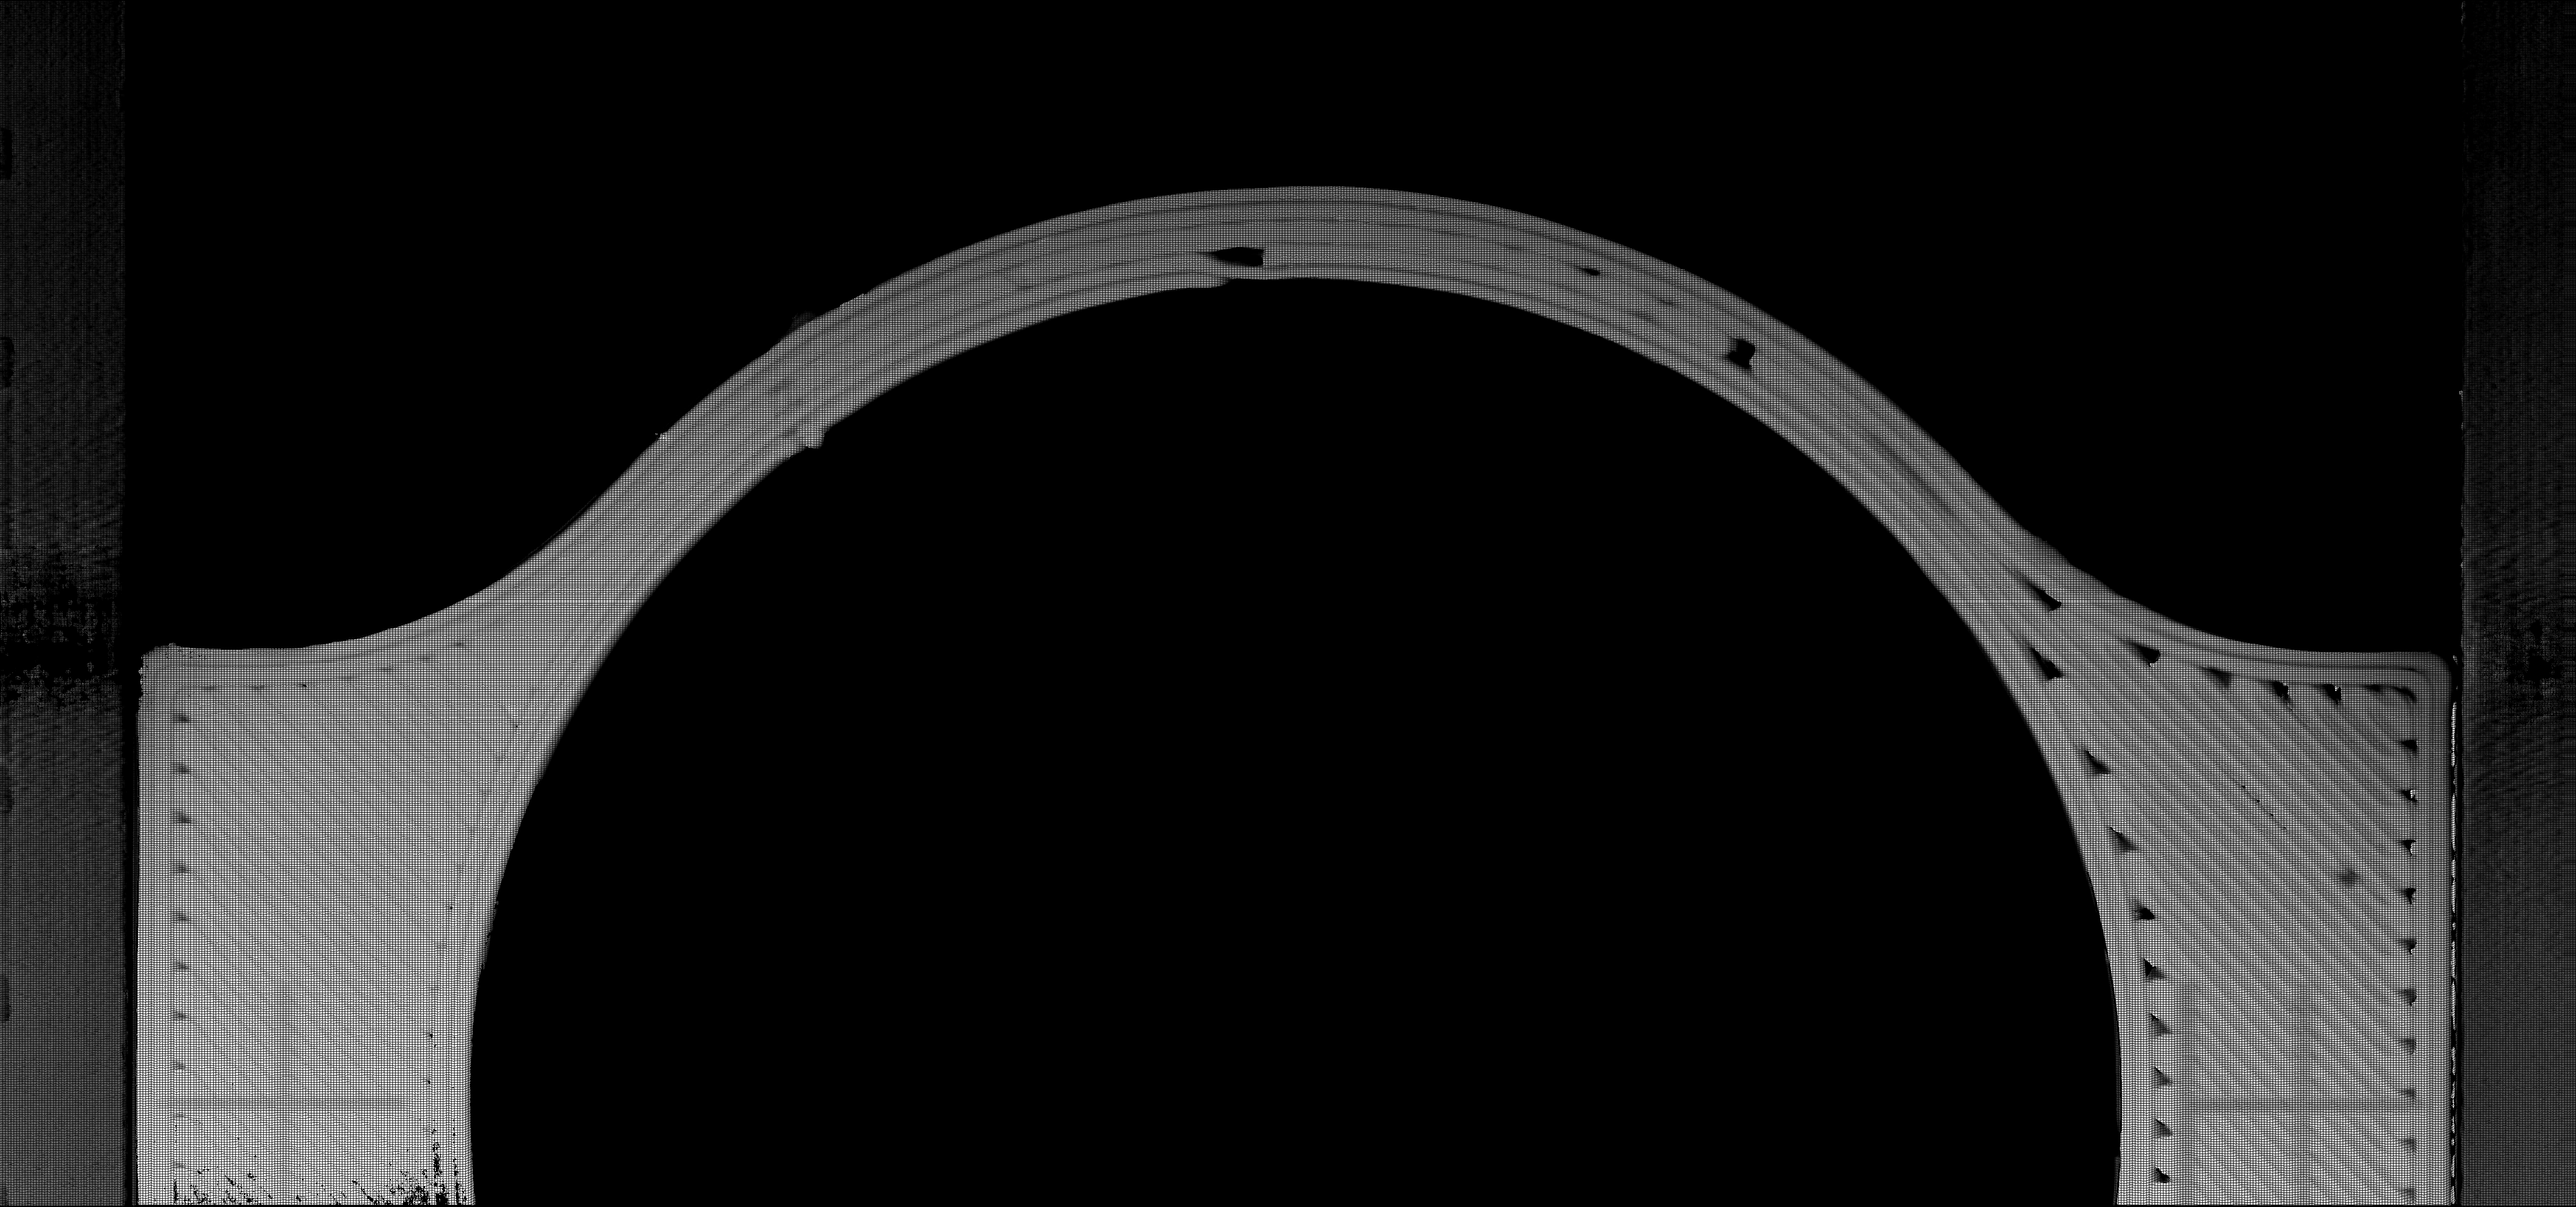
\includegraphics[width=0.95\textwidth]{images/fdm_top_10p.png}
    \caption{Resultat der Pointcloud zu Bild Konvertierung eines FDM Bauteils}
    \label{fig:10p}
\end{figure}


\chapter{Stitching}

Für jeden Einspannzustand eines Bauteils können mehrere Bilddateien vorliegen.
Alle Bilddateien gehören zu dem gleichen Bauteil und müssen 
zusammengefügt werden, um ein einzelnes digitales Objekt zu erhalten. 
Als Voraussetzung ist gegeben das alle Bilder Überlappung enthalten.

Diese Überlappung kann benutzt werden, um die Bilder zu einem Objekt zusammenzufügen.
Das Zusammenfügen ist im folgenden auch Stitching genannt.
Für das Stitching von Bilddateien existieren schon mehrere Verfahren die in Bibliotheken
für viele Programmiersprachen implementiert sind. Der schon beschriebene ICP-Algorithmus
ist eines dieser Verfahren. Das Problem mit diesen Verfahren ist das sich zwei 
Datensätze angenähert werden indem auf ein Datensatz so lange eine 
Transformation und Rotation, manchmal auch eine Skalierung, angewendet wird, bis
die Distanz der Datensätze unter einen Grenzwert fällt oder nicht mehr verbessert
werden kann. Die Überlappung in den von dem Laserscanner aufgenommen Daten ist jedoch 
nur in zwei Achsen verschoben. Durch eine Rotation der Daten wird eine nicht korrekte 
Distanz berechnet.
Um die korrekte Transformation zu finden, mit der die beiden Bilder überlappen
muss nicht der komplette Bereich analysiert werden, sondern nur der überlappende Teil.
In diesem Bereich müssen Features erkannt werden. 
Nachdem in beiden Teilbildern Features erkannt wurden können diese miteinander
verglichen werden.

\section{Feature Erkennung}

Features in einem Bild sind große Unterschiede in benachbarten Pixeln. Die größten
Features sind die Ränder des Bauteils, kleinere Features können Oberflächenänderungen 
oder Spuren des Herstellungsprozesses sein. Diese Unterschiede können mithilfe 
der 'OpenCV' Bibliothek extrahiert werden. Diese Bibliothek gibt die erkannten 
Features als Liste von Konturen aus. Konturen selbst bestehen aus Listen von 
Punkten, die aus X und Y Koordinaten bestehen. Die Konturerkennung kann verbessert 
werden, indem das Bild entsprechend präpariert wird. In Abbildung \ref{fig:cons} und
\ref{fig:image_top} ist ein Ursprungsbild und die extrahierten Konturen zu sehen.
Mittig am linken und rechten Rand sind in Abbildung \ref{fig:image_top} 
Messfehler des Laserscanners zu sehen. Diese werden auch als Features in 
Abbildung \ref{fig:cons} erkannt. Diese müssen entfernt werden damit die Bilder 
korrekt zusammengefügt werden können. Erfolgt dies nicht werden diese Fehler miteinander
verglichen was das Ergebnis verfälscht.

\begin{figure}[h]
    \centering
    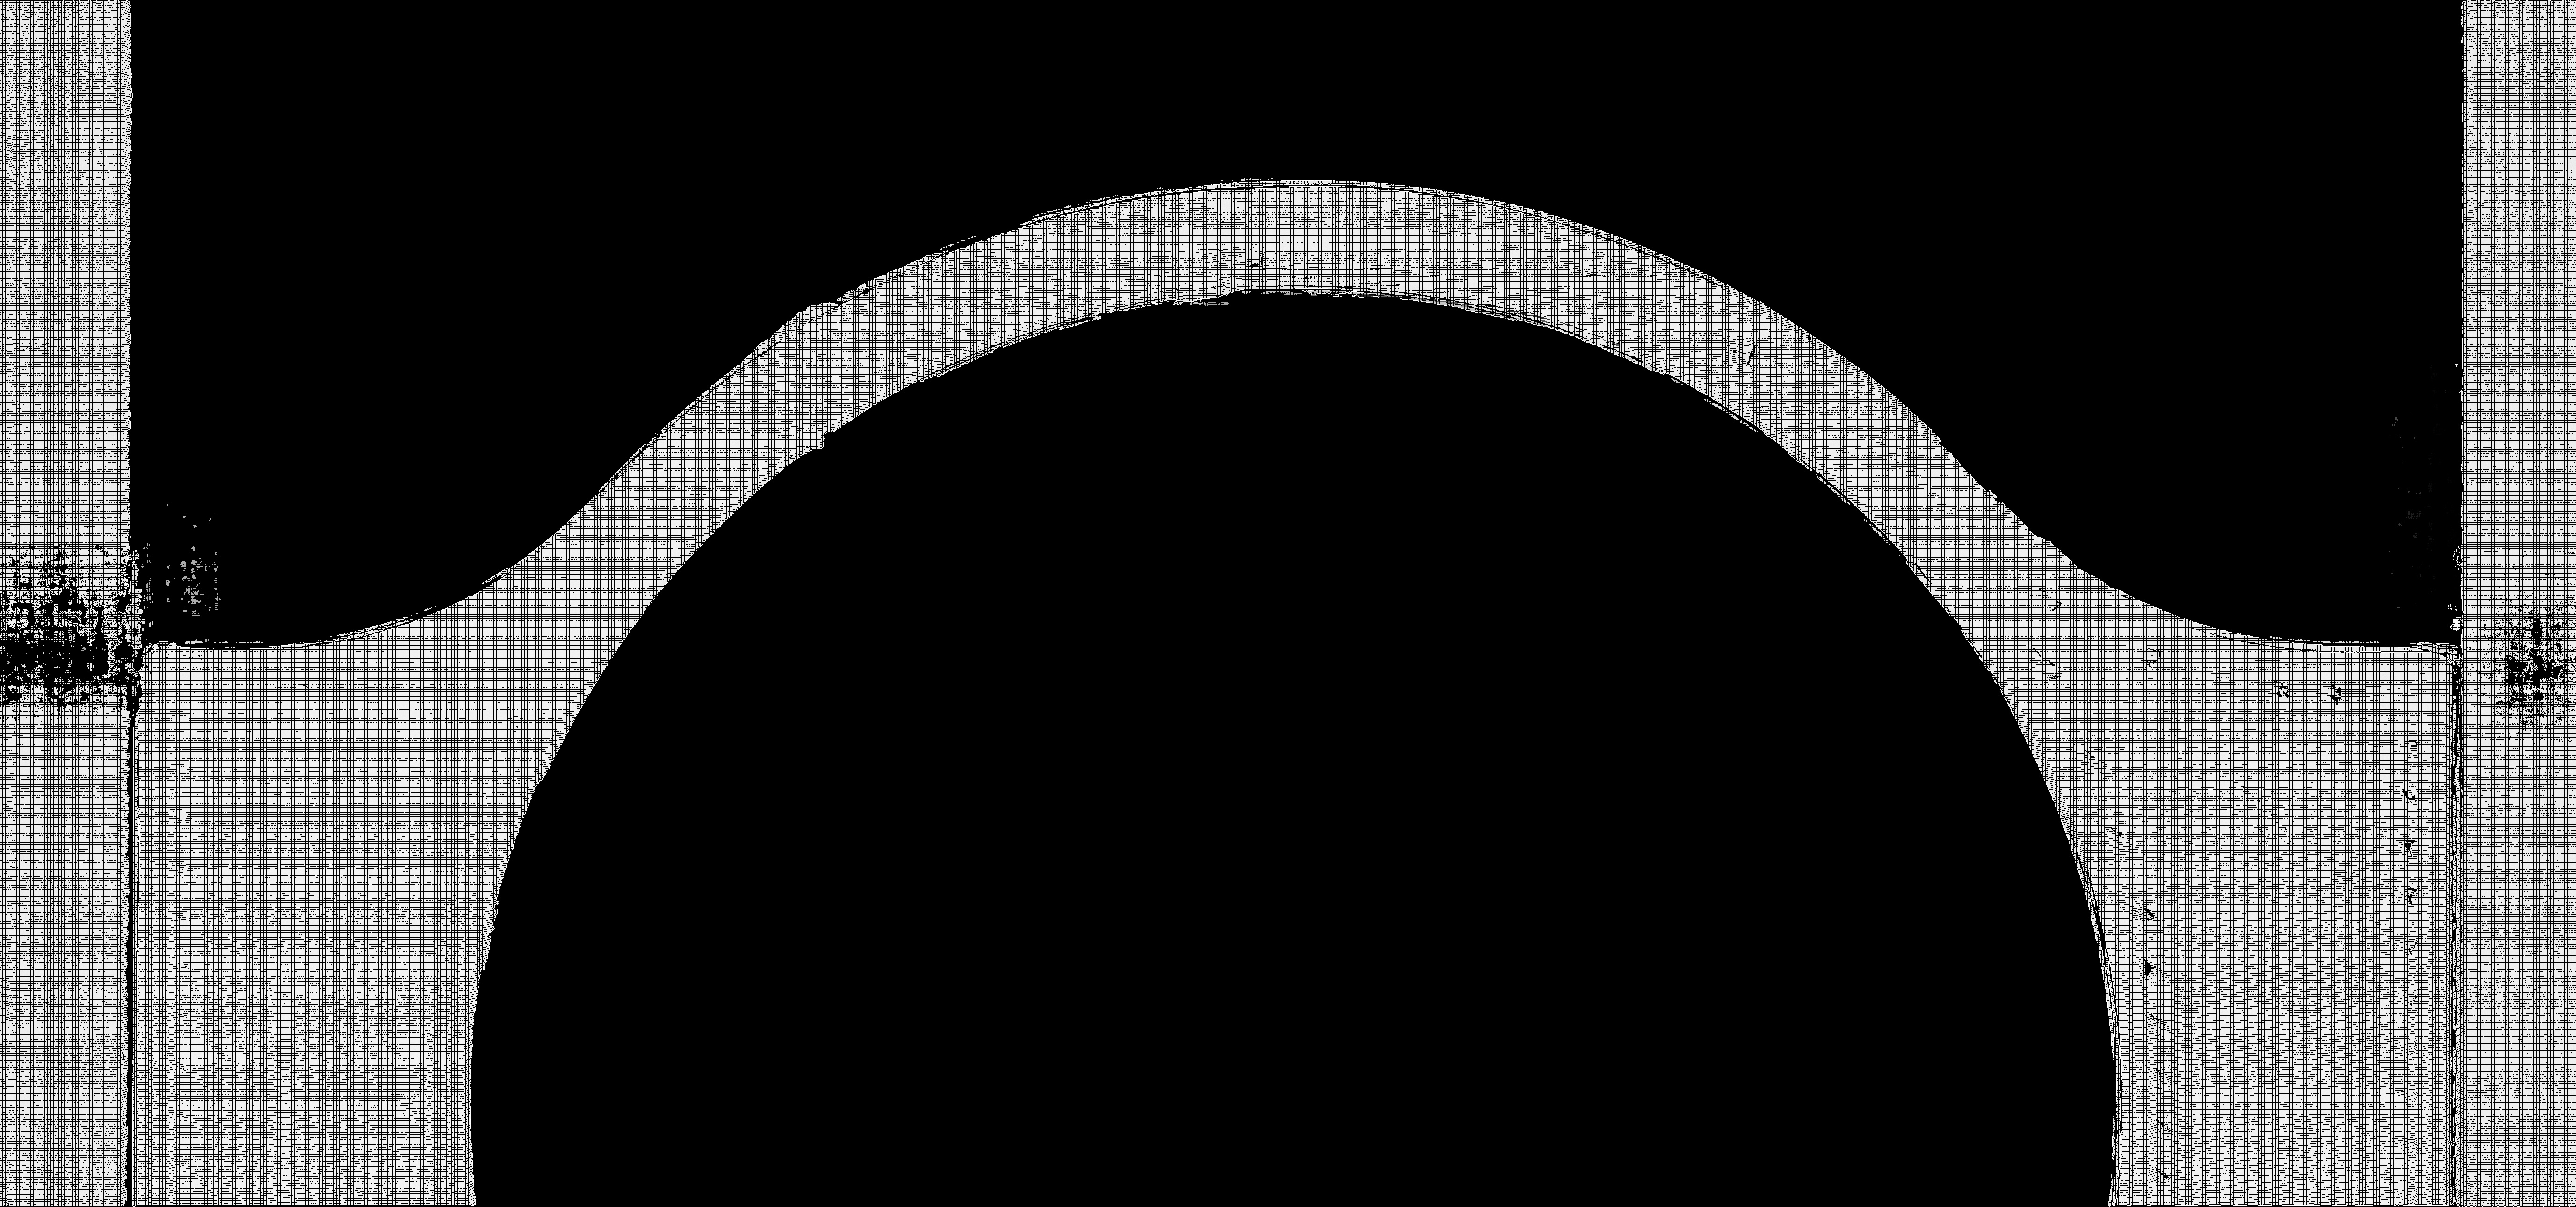
\includegraphics[width=0.8\textwidth]{images/with_con.jpg} % first figure itself
    \caption{Oberes Bild eines Scanvorgangs, FDM Bauteil}
    \label{fig:image_top}
\end{figure}

\begin{figure}[h]
    \centering
    \includegraphics[width=0.8\textwidth]{images/only_con.jpg} % second figure itself
    \caption{Extrahierte Kontouren des Bildes ohne Pre-Processing}
    \label{fig:cons}
\end{figure}

Die Überlappung kann nur im oberen oder unteren Bildbereich auftreten. Der restliche 
Teil des Bildes kann also entfernt werden. So wird außerdem Rechenzeit gespart.

\begin{figure}[h]
    \centering
    \includegraphics[width=0.8\textwidth]{images/only_con_cut.jpg} % second figure itself
    \caption{Extrahierte Kontouren des Bildes ohne Pre-Processing, zugeschnitten 
    auf den (vermutlich) überlappenden Bereich}
    \label{fig:cons_cut}
\end{figure}

Dieses Verfahren wird auf beide Bilder angewendet. Daraus resultieren dann zwei 
zugeschnittene Bilder aus denen Konturen extrahiert wurden. 
Würden diese beiden Bildteile vollständig überlappen könnte jetzt der ICP-Algorithmus
angewendet werden. Dieser würde dann die korrekte Transformation berechnen in dem er 
die Konturen aus dem oberen Bild, mit denen aus dem unteren Bild vergleicht und die 
Distanz zwischen den Punkten minimiert. 
Der Grad der Überlappung ist unbekannt und kann nicht im Vorhinein bestimmt werden.
Dadurch kann der ICP-Algorithmus nicht eingesetzt werden. 
Eine andere wichtige Annahme kann getroffen werden: Jeweils eine Kontur aus 
dem oberen und unteren Bild haben mindestens einen gemeinsamen Punkt.

\section{Differenzierung von Punkten}

Die Distanz zwischen zwei Punkten kann über den euklidischen Abstand gemessen werden.
\cite{Dokmanic.2015}. Sei A ein Punkt in einer Kontur aus dem oberen Bild und K eine 
Kontur aus dem unteren Bild.  
Um den Punkt aus K zu finden, der am nächsten an A liegt, muss A mit jedem Punkt aus 
K verglichen werden. Das Punktepaar mit dem kleinsten gefunden Euklidischen Abstand 
wird als 'Best Match' gespeichert. Wenn die Euklidische Distanz null beträgt, kann 
die Suche abgebrochen werden, da kein kleinerer Wert mehr gefunden werden kann.
Dieser Ansatz ist dem ICP-Algorithmus ähnlich. Die Differenz zwischen zwei Konturen 
K1 und K2 kann verglichen werden, indem für jeden Punkt A aus K1 der näheste Punkt aus 
K2 gefunden wird. In dem ICP-Algorithmus werden alle Distanzen von der 'Best Matches' 
aufsummiert und beschreiben den Unterschied der beiden Distanzen. Diese Summe kann dann 
minimiert werden. Dieser Ansatz funktioniert bei einem sich nur partiell
überlappenden Datensatz nicht. 
Statt die Summe zu bilden, wird jede beste Distanz zusammen mit ihren korrespondieren 
Punkten gespeichert. Um den Grad der Überlappung zu bestimmen, werden die Distanzen 
gezählt die gleich null sind. Dieser Wert in Relation zu der Länge von K1 gibt, 
in Prozent, an zu welchem Anteil sich die beiden Konturen überlappen.

\section{Transformation bestimmen}

Gesucht ist die Transformation welche die maximale Überlappung der beiden 
Konturen K1 und K2 bietet. Um diese Transformation zu berechnen, muss der 
Grad der Überlappung für jede mögliche Positionierung ermittelt werden. Jeder
Punkt aus K2 muss auf die Koordinaten eines beliebigen aber festen Punkts aus K1 
verschoben werden.
Die Transformation zwischen zwei Punkten A und B kann über die Vektorberechnung erfolgen:

\begin{equation*}
    T_{a,b} = \begin{pmatrix}a_x\\a_y\end{pmatrix} - \begin{pmatrix}b_x\\b_y\end{pmatrix}
\end{equation*}

Kontur K2 kann über Kontur K1 verschoben werden, indem Punkt A festgehalten wird, 
während Punkt B sukzessive jeden Punkt aus K2 annimmt. 
Die daraus resultierende Punkttransformation wird auf jeden Punkt von K1 angewendet, 
um die nächstgelegenen Nachbarpunkte zu ermitteln. Für jede Transformation wird der 
Überlappungsanteil berechnet, wobei das Ergebnis mit der maximalen Überlappung
als die optimale Transformation gespeichert wird.
Dieses Verfahren ist nur anwendbar, wenn Punkt A im überlappenden Bereich liegt. 
Befindet sich Punkt A nicht in der Kontur K2, 
kann das Verfahren nicht erfolgreich angewendet werden.
Zur Berechnung der optimalen Transformation werden verschiedene Punkte aus K1 
ausgewählt und das Verfahren jeweils angewendet. 
Die Transformation mit dem größten Verhältnis von Nullen zur
Gesamtlänge der Kontur wird als optimal angesehen. 
Aufgrund des exponentiellen Laufzeitverhaltens ist es ineffizient, 
jeden Punkt A aus K1 mit jedem Punkt B aus K2 zu vergleichen.

In Abbildung \ref{fig:before_matching} sind zwei Beispielkonturen zu sehen. 
Diese sind nicht angeordnet. Der ICP-Algorithmus würde diese beiden Konturen 
annähern, ohne sie zu überlappen. 
Das Ergebnis des vorgestellten Stitching Verfahrens ist in Abbildung 
\ref{fig:after_matching} zu sehen. Es ist zu erkennen das, trotz Messfehler und 
kleineren unterschieden im überlappenden Bereich die korrekte Transformation 
ermittelt werden konnte. Diese Konturen stammen von einem additiv gefertigten 
Metallbauteil.

\begin{figure}[h]
    \centering
    \begin{minipage}{0.49\textwidth}
        \centering
        \includegraphics[width=\textwidth]{images/before_matching.png} % first figure itself
        \caption{Konturen, vor der Transformation}
        \label{fig:before_matching}
    \end{minipage}
    \begin{minipage}{0.49\textwidth}
        \centering
        \includegraphics[width=\textwidth]{images/0.24225865209471767contours.png} % first figure itself
        \caption{Konturen, transformiert mit größter Überlappung, 
        Grad der Überlappung: 24,26\%}
        \label{fig:after_matching}
    \end{minipage}\hfill
\end{figure}

\section{Stitching visuell dargestellt}

In Abbildung \ref{fig:stitching_all} ist der Prozess des Verfahrens zu sehen.
K1 ist in Blau dargestellt, K2 in Grün.
In jeden Bild ist der Grad der Überlappung dargestellt. Es ist dargestellt wie
Kontur K2 über K1 geschoben wird, um den besten Grad der Übereinstimmung zu ermitteln.
Die Bilder sind repräsentativ ausgewählt, im tatsächlichen Prozess wird K1 komplett 
über K2 bewegt.

\begin{figure}[h]
    \centering
    \begin{minipage}{0.24\textwidth}
        \centering
        \includegraphics[width=\textwidth]{images/stitching_beginn.PNG} % first figure itself
        \caption*{(a)}
    \end{minipage}
    \begin{minipage}{0.24\textwidth}
        \centering
        \includegraphics[width=\textwidth]{images/stitching_middle.PNG} % first figure itself
        \caption*{(b)}
    \end{minipage}\hfill
    \begin{minipage}{0.24\textwidth}
        \centering
        \includegraphics[width=\textwidth]{images/stitching_match.PNG} % first figure itself
        \caption*{(c)}
    \end{minipage}\hfill
    \begin{minipage}{0.24\textwidth}
        \centering
        \includegraphics[width=\textwidth]{images/stitching_end.PNG} % first figure itself
        \caption*{(d)}
    \end{minipage}\hfill
    \caption{Verfahren im Verlauf dargestellt, a am Anfang, b nach n-durchgängen, c }
    bei einem guten Match, d Kontur K2 komplett über K1 geschoben.
    \label{fig:stitching_all}
\end{figure}


\section{Bilder zusammenfügen}

Wenn alle Transformationen vorliegen wird die Transformation mit der besten 
Übereinstimmung gewählt. Diese wird genutzt, um die beiden Bilder zusammenzufügen.
Das zugehörige Bild der Konturen K2 wird transformiert, indem die Transformation 
auf jeden Pixel angewendet wird.  
Die Transformation ist nur korrekt, wenn die beiden Bilder die gleichen 
Ursprungskoordinaten haben, die auch bei den Konturen K1 und K2 verwendet wurden.

\begin{figure}[h]
    \centering
    \includegraphics[width=0.8\textwidth]{images/AM_SP0_stitched_2.png} % first figure itself
    \caption{Zusammengefügtes Bild}
    \label{fig:stitched_image}
\end{figure}

\section{Probleme und Lösungen im Verfahren}

Durch die Funktionsweise treten am Randbereich der Scannerdaten vermehrt Messfehler auf, 
die nicht vollständig durch vorheriges Filtern entfernt werden können. 
Damit diese Messfehler das Stitching nicht verfälschen, werden alle Konturen nochmals 
gefiltert. Alle Punkte in einer Kontur, die sich in einem konfigurierbaren 
Abstand zu den Bildrändern befinden, werden entfernt. Dadurch werden sie bei der 
Berechnung der Transformation nicht verwendet. 
Der konfigurierbare Abstand muss beim Stitching des finalen Bilds berücksichtigt 
werden und von der Transformation abgezogen werden.

Wenn Konturen mit einem großen Längenunterschied verglichen werden, 
kann eine sehr hohe Übereinstimmung ermittelt werden, die aber keine 
tatsächliche Übereinstimmung ist. Dies liegt daran, dass es wahrscheinlicher ist 
eine Sequenz der Länge 5 in einer anderen Sequenz der Länge 500 zu finden.  
Das kann zum Beispiel vorkommen, wenn Konturen 
die am linken und rechten Bildrand in Abbildung \ref{fig:cons} zu sehen sind, 
verglichen werden. Um dies zu vermeiden wird eine Bedienung eingeführt, dass die Länge
der Konturen nicht zu sehr voneinander abweichen darf. Bei einer Abweichung von mehr als
200 Punkten in einer Kontur sollte die Konturen nicht miteinander verglichen werden.

Auch Konturen mit einer Länge von weniger als 100 Punkten sollten nicht berücksichtigt 
werden. Diese beschreiben keine Features in einem Bild, die für das Stitching verwendet 
werden sollten. Diese Konturen beschreiben meist nur Messfehler oder 
Oberflächenstrukturen, die nicht konsistent in beiden Bildern von dem Scanner erkannt 
werden können.

Um das Ergebnis noch weiter zu verbessern, können zwei Konturen zweimal miteinander 
verglichen werden. Während des zweiten Vergleichs wird die Zielkontur mit der 
Ursprungskontur vertauscht. So wird aus beiden Konturen jeweils einmal ein fester 
Punkt gewählt. Wieder wird die Transformation gespeichert mit der besten Überlappung.
Wenn die Überlappung im zweiten Vergleich eine höhere Übereinstimmung hat, muss die 
berechnete Transformation invertiert werden. Geschieht dies nicht, kann die 
Transformation nicht für den finalen Stitchprozess eingesetzt werden, weil dort 
das Ziel und Ursprungsbild fest gesetzt ist.


\chapter{Analyse der spannkraftinduzierten Deformation}




\chapter{Validierung}

Im folgenden Kapitel wird die Deformationerkennung analysiert und überprüft.
Zur Überprüfung werden Materialeigenschaften und aufgenommene Messwerte 
mit der erkannten Deformation verglichen.

\section{Messergebnisse}

Es wurden fünf Bauteile mit verschiedenen Spannungsstufen gemessen. Für jede 
Spannungsstufe wurde die Kraft, die auf das Bauteil wirkte sowie die Verschiebung 
des Schraubstocks gemessen.
Jede Spannungsstufe wurde durch Stufenweises anziehen des Schraubstocks erreicht.
Die Spannkraftkurve eines einzelnen Einspannvorgangs ist in 
Abbildung \ref{fig:single} zu sehen. 
In der Spannungskurve ist ein elastischer Bereich für das 
Bauteil zu sehen, in dem sich die Spannkraft zurückbewegt, nachdem kein 
Anzugdrehmoment mehr anliegt. Aus diesem Grund kann nicht der maximale Wert der Spannkraft angenommen werden, 
sondern es muss ein Wert gewählt werden der nach dem maximalen Ausschlag liegt.
Dieser wurde über die erste Ableitung der Spannkraftkurve gefunden. Sobald der 
Absolutwert der Steigung unter 0.0009 N fällt, wir die Spannkraft und Auslenkung an 
diesem Punkt gewählt. 0.0009 N wurde empirisch ermittelt, um bei allen Bauteilen einen 
angemessenen Wert zu liefern.
Die Spannkraft wurde an zwei Achsen aufgenommen und zu der Gesamtkraft aufsummiert.

\begin{figure}[H]
    \centering
    \includegraphics[width=0.99\textwidth]{images/spannkraftstufen_single.png}
    \caption{Kraft- und Verschiebung der Spannungsstufe fünf bei einem FDM Bauteil}
    \label{fig:single}
\end{figure}

Diese maximalen Werte für die Spannkraft und Auslenkung wurden für jedes Bauteil 
akkumuliert und sind in Abbildung \ref{fig:akkumulated} dargestellt. 
Die mit dem FDM-Prozess hergestellten Bauteile wurden jeweils in sechs Spannungsstufen
gemessen. Zwischen den Stufen wurde versucht, eine konstante Kraft auf das Bauteil 
auszuüben. Durch den manuellen Prozess des Anziehens des Schraubstocks war dies 
jedoch nicht immer möglich.
Die Metallbauteile unterscheiden sich durch ihren Aufbau. 
Alle basieren auf dem gleichen 3D-Modell, besitzen jedoch unterschiedliche 
Stützstrukturen. Im Bauteil AM0 ist die vollständige Stützstruktur vorhanden,
während in den Bauteilen AM1 und AM2 die Stützstruktur in unterschiedlicher 
Tiefe ausgebohrt wurde. Die Bauteile sind in Abbildung \ref{fig:am_parts} dargestellt.

Das Bauteil AM0 wurde nur mit zwei Spannungsstufen gemessen, 
da bereits bei der zweiten Stufe über 2500 N Kraft erforderlich war, 
um das Bauteil nur minimal in x-Richtung zu deformieren. Dies zeigt, 
dass die Stützstruktur einen erheblichen Einfluss auf die Verformbarkeit 
eines Bauteils hat. Beim Bauteil AM1 wurden 2500 N erst nach vier Spannungsstufen 
erreicht. Vergleicht man die Verformung in x-Richtung mit der Verformung von AM2,
 zeigt sich, dass das Bauteil ohne Stützstruktur bei ähnlicher Krafteinwirkung 
 etwa doppelt so weit in x-Richtung deformiert wurde.

 Die FDM-Bauteile wurden mit deutlich weniger Kraft eingespannt. 
 Hier wurde bei etwa 250 N gestoppt, dennoch ist die Verschiebung der 
 Teile deutlich größer als bei den AM-Bauteilen. Diese Werte wurden aufgenommen, 
 um die visuelle Deformationserkennung zu validieren.

\begin{figure}[H]
    \centering
    \includegraphics[width=0.99\textwidth]{images/spannkraftstufen_akkumuliert.png}
    \caption{Akkumulierte Kraft und Verschiebung, mit der jedes Bauteil deformiert wurde.}
    \label{fig:akkumulated}
\end{figure}

\begin{figure}[H]
    \centering
    \begin{minipage}{.33\textwidth}
      \centering
      \includegraphics[width=0.9\linewidth]{images/AM0_crop.JPG}
      \caption*{(a)}
    \end{minipage}%
    \begin{minipage}{.33\textwidth}
      \centering
      \includegraphics[width=0.9\linewidth]{images/AM1_crop.JPG}
      \caption*{(b)}
    \end{minipage}
    \begin{minipage}{.33\textwidth}
        \centering
        \includegraphics[width=0.9\linewidth]{images/AM2_crop.JPG}
        \caption*{(c)}
      \end{minipage}
      \caption{(a): AF Metallbauteil mit voller Stützstruktur, Bezeichnung: AM0.
      (b): AF Bauteil mit der halben Stützstruktur ausgebohrt, Bezeichnung: AM1.
      (c): AF Bauteil ohne Stützstruktur, Bezeichnung: AM2}
      \label{fig:am_parts}
\end{figure}

\section{Ergebnisse der optischen Deformationsanalyse}

In Abbildung \ref{fig:am_defos} und Abbildung \ref{fig:fdm_defos} sind die erkannten,
vertikalen Deformation grafisch dargestellt. Jeweils von Spannungsstufe null bis 
Spannungsstufen Sechs. Bei dem FDM Bauteil fehlt die Spannungsstufen fünf, 
diese ist leider bei der händischen Dateiname Vergabe überschrieben worden und konnte 
deshalb nicht ausgewertet worden. Aus diesem Grund ist eine so große Lücke in der 
Abbildung \ref{fig:fdm_defos}.
Außerdem sind große Unterschiede in der absoluten Deformation zu sehen. Zum Beispiel 
die rote Kurve in Abbildung \ref{fig:am_defos} die den Unterschied der Spannungsstufen 
null und eins angibt. Diese Kurve sollte näher an null der y-Achse liegen. 
Dies liegt an Ungenauigkeiten in dem Stitching Verfahren. In den Graphen ist also 
auf die Steigung der Deformationskurve zu achten. In der Steigung erkannt man das 
sich die Bauteile in mittleren Bereich nach außen hin deformiert haben und in 
den Randbereichen sich nach innen und dann wieder nach außen deformieren.
Außerdem ist im Vergleich der beiden Graphen zu sehen das sich das FDM Bauteil deutlich 
mehr verformt hat. Hier beträgt die größte Deformation über 150 Pixel.
Bei dem Metallbauteil, das mit der zehnfachen Kraft eingespannt wurde (250 nm vs. 2500 nm)
sind es nur knapp 40 Pixel, wie in Abbildung~\ref{fig:deformation_data_am} zu sehen. Trotzdem ist zu sehen das sich die Bauteile, die auch die 
gleiche Geometrie teilen, auf die gleiche Weise verformt haben.

\begin{figure}[H]
  \centering
  \includegraphics[width=0.95\textwidth]{images/am2_all_defos.png}
  \caption{Sechs Deformationsstufen bei einem additiv gefertigten Metallbauteil ohne
  Stützstruktur von 0 bis 2500 nm}
  \label{fig:am_defos}
\end{figure}

\begin{figure}[H]
  \centering
  \includegraphics[width=0.95\textwidth]{images/fdm2_all_defos.png}
  \caption{Fünf Deformationsstufen bei einem FDM Bauteil von 0 bis 250 nm}
  \label{fig:fdm_defos}
\end{figure}

\begin{figure}[H]
    \centering
    \includegraphics[width=0.9\textwidth]{images/AM_sp0_sp2_defo_plot.png}
    \caption{Differenz von zwei Spannungsstufen bei einem additiv gefertigten Metallbauteil, 
    das zur Hälfte mit Stützstrukturen gefüllt ist (Abbildung~\ref{fig:am_parts (b)}). }
    \label{fig:deformation_data_am}
\end{figure}

\section{Beurteilung der Ergebnisse}

Grundsätzlich ermöglicht die Methode die Erkennung und den Vergleich von Deformationen 
eines Bauteils. Die gemessene Deformation eines Bauteils entspricht den erwarteten Werten, 
abhängig von Material und Geometrie des Bauteils. FDM-gedruckte Kunststoffteile zeigen 
eine deutlich stärkere Verformung im Vergleich zu Metallteilen.
Bei den Metallteilen zeigt sich, dass das Vorhandensein einer Stützstruktur die
Verformung des Bauteils signifikant reduziert. 
Die unterschiedlichen Deformationen sind in Abbildung \ref{fig:materials} dargestellt. 
Das in Abbildung \ref{fig:am_parts} (a) gezeigte Bauteil konnte nicht analysiert werden, 
da durch die Stützstruktur keine korrekte Transformation zur stitchen berechnet werden konnte.
Bei den FDM-Bauteilen ist festzustellen, dass sie sich deutlich stärker verformen 
als die Metallteile. Beide FDM-Bauteile zeigen eine ähnliche Verformungsausprägung, 
jedoch tritt die Deformation, trotz identischer Geometrie, an unterschiedlichen Stellen auf. 
Dies könnte auf Unterschiede im Druckprozess zurückzuführen sein. 
Diese Beobachtung zeigt einen weiteren Nutzen der Methodik: Sie ermöglicht
nicht nur die Bestimmung des Ausmaßes der Deformation, sondern auch die 
Identifikation von Schwachstellen innerhalb eines Bauteils, die zu einer erhöhten 
 
Deformation führen.

\begin{figure}[H]
  \centering
  \includegraphics[width=0.95\textwidth]{images/compare_materials.png}
  \caption{Vergleich von Materialien und Bauteilgeometrien}
  \label{fig:materials}
\end{figure}

Dennoch ist die Deformationserkennung noch nicht perfekt. 
Fehler im Stitching Prozess führen zu starken Änderungen in der Deformationserkennung. 
Wie in Abbildung \ref{fig:errors} zu sehen ist, kann sich die Breite des Bauteils 
zwischen zwei Spannungsstufen unterscheiden. Er ist erkennbar, dass der Rand der einen 
Kontur, repräsentiert durch die magenta gefärbte Linie, immer größer ist als 
der Rand der anderen Kontur, hier in blau dargestellt.
Dieser Versatz entsteht, weil beim Stitching eine Transformation verwendet wurde die sich 
um wenige Pixel unterscheidet. Dadurch wächst auch die erkannte Deformationen.
Aus diesem Grund existieren in den Abbildungen \ref{fig:am_defos} und \ref{fig:fdm_defos}
Linien die nicht dem erwarteten Verhalten entsprechen. 
In Abbildung \ref{fig:fdm_defos} zum Beispiel, sollte die Deformation zwischen den 
Spannungsstufen eins und zwei 
(in rot dargestellt) am kleinsten sein. Stattdessen liegt die Kurve bei -50 Pixeln im Graph.

\begin{figure}[H]
  \centering
  \includegraphics[width=0.95\textwidth]{images/contours_matching_36.png}
  \caption{Vergleich von Konturen aus nicht korrekt zusammengefügten Bildern.}
  \label{fig:errors}
\end{figure}

Zusätzlich kann, bei Bildern ohne klare Konturen, das Stitching nicht korrekt durchgeführt
werden. Dies ist bei den additiv gefertigten Metallbauteil mit Stützstruktur der Fall 
(Abbildung \ref{fig:am_parts} (a)). Das Bild, das aus dem Scan dieses Bauteils erstellt wurde, 
ist in Abbildung \ref{fig:errorimage} zu sehen. Es lassen sich keine eindeutigen Konturen 
erkennen, die für das Stitching genutzt werden könnten.

\begin{figure}[H]
  \centering
  \includegraphics[width=0.95\textwidth]{images/am0.png}
  \caption{Bild eines Scans von einem Metallbauteil mit Stützstruktur.}
  \label{fig:errorimage}
\end{figure}




\chapter{Anwendung und Algorithmus}

Ziel dieser Arbeit ist es nicht nur eine Methodik zur optische 
Deformationserkennung zu entwickeln, sondern diese Methodik auch in einer 
Anwendung einfach nutzbar zu machen. 

Diese Kapitel dokumentiert diese Anwendung und geht auf Herausforderungen 
in der Entwicklung ein.

\section{Anwendung}

Die Anwendung beinhaltet verschiedene Funktionen, alle Funktionen 
können separat benutzt werden. Dadurch müssen zeitintensive Vorgänge nicht 
wiederholt werden, sondern Zwischenergebnisse können abgespeichert und 
neu geladen werden.
Die Anwendung bietet Funktionen, um Resultate in dem entsprechenden Dateiformat zu 
speichern. Soweit möglich werden Dateinamen Empfehlungen automatisch ermittelt, 
daher ist es zu empfehlen von Anfang an mit einem einheitlichen Namensschema bei
den 3D-Scannerdaten zu arbeiten. 
Das Schema \glqq Bauteilbeschreibung \textunderscore Spannungsstufe\grqq~~
\textunderscore Scannerdurchlauf.ply
wird empfohlen. Ein Beispiel für die zweite Pointcloud eines FDM-Bauteil bei der
vierten Spannungsstufen wäre also \glqq FDM0\textunderscore SP4\textunderscore 2.ply\grqq~.
In Abbildung \ref{fig:software_screenshot} ist die Oberfläche der Anwendung zu sehen.

\begin{figure}[H]
    \centering
    \includegraphics[width=0.9\textwidth]{images/software_screenshot.png}
    \caption{Anwendungsoberfläche}
    \label{fig:software_screenshot}
\end{figure}

Über die Buttons \glqq Select Pointcloud\grqq~ können Pointclouds zum Konvertieren in Bilder
ausgewählt werden. Der Text neben dem Bild zeigt den Dateinamen der ausgewählten 
Datei an. Die obere Pointcloud sollte hier als erstes ausgewählt werden.
Der Button \glqq Start PC conversion\grqq~~startet die Konvertierung. Der Balken 
daneben zeigt den Prozessfortschritt. 
Wenn \glqq Show Pointclouds\grqq~ gesetzt ist, werden die Pointclouds vor dem 
Konvertieren in einem separaten Fenster angezeigt. So kann überprüft werden, ob die 
korrekte Pointcloud ausgewählt wurde.
Wenn der Prozess abgeschlossen ist, werden die resultieren Bilder als Vorschau in der 
Anwendung angezeigt und die Option zum Speichern der Bilder ist nicht mehr ausgegraut.
Zusätzlich wird nach dem Konvertierungsprozess die Schaltfläche 
\glqq Stitch converted\grqq~ freigeschaltet. Durch diese Option können die 
Bilder direkt zusammengefügt werden, ohne das die Bilder extra gespeichert und 
eingeladen werden müssen. Wenn schon existierende Bilder zusammengefügt werden sollen, 
können die Schaltflächen \glqq Select top image\grqq und \glqq Select bot image\grqq
ausgewählt werden um das obere und untere Bild auszuwählen. Auch hier wird die 
ausgewählte Datei als Text angezeigt. Die Dateiauswahl erfolgt über das 
Windows-Kontextmenü, der zuletzt verwendete Ordner wird hierbei erhalten, sodass das 
zweite Bild schneller ausgewählt werden kann. 
Über den Button \glqq Start stitching\grqq wird der stitching Prozess gestartet. 
Auch hier wird der Fortschritt und das Endresultat, sobald es vorliegt, angezeigt.

Damit auch die CAD-Datei des additiv gefertigten Bauteils verglichen werden kann, 
existiert der \glqq Convert stl\grqq~ Button. Hier wird eine .stl Datei zu einem Bild 
konvertiert und kann über \glqq save stl\grqq~ gespeichert werden.

Mithilfe der rechts zu sehenden Schaltflächen können Bilder auf ihre Deformation hin 
verglichen werden. Die resultieren Deformationsdaten werden automatisch als Textdatei
in dem Ordner \glqq deformation\underline data\grqq~ gespeichert. Dieser Ordner wird automatisch 
in dem Verzeichnis erzeugt, in dem die Anwendung ausgeführt wird. 
Die erstellten Textdateien können mithilfe des Buttons \glqq Plot data\grqq~ ausgewählt 
werden, und werden automatisch als Graph angezeigt. 

Beim Konvertieren und stitchen werden alle Prozesse, die nicht voneinander abhängig sind,  
nebenläufig ausgeführt. Das reduziert die Laufzeit der Prozesse.

Die Anwendung ist in Python geschrieben, rechenintensive Prozesse wurden aber mithilfe 
der Bibliothek \glqq Numba\grqq~in optimierten Maschinencode compiliert~\cite{numba}.
Dadurch ist der Konvertierungs- und Stitching-Prozess deutlich schneller geworden. 
Durch die Optimierungen konnte der Konvertierungsprozess von 49 s auf 41 s verschnellert 
werden. Bei dem Stitchprozess war die Verbesserung noch deutlicher. Hier 
beträgt die Laufzeit mit Optimierungen ca. 30 s um zwei Konturen zu vergleichen. 
Ohne Optimierungen braucht der Vergleich derselben beiden Konturen 
hochgerechnet 600 Minuten.





\chapter{Zusammenfassung und Ausblick}

[Stichpunkte]

\begin{itemize}
    \item Auf die Unterschiede der Materialen eingehen. Auch auf die ähnlichkeiten 
    wo die Deformation auftreten.
    \item Was das für die Bauteile bedeutet.
    \item Verbesserung: Stitching verbessern um einheitlichere Ergebnisse zu erhalten.
    \item Forschungsansätze: Veränderung in der inneren Struktur der Bauteile 
    vergleichen.
\end{itemize}

% Anhang
\appendix
% Abbildungsverzeichnis
\listoffigures
\addcontentsline{toc}{chapter}{Abbildungsverzeichnis}
\cleardoublepage
% Literaturverzeichnis
\bibliographystyle{alpha}
\bibliography{literatur/quellen}
\addcontentsline{toc}{chapter}{\bibname}
% Erklaerung
\thispagestyle{myheadings}
\end{document}

